\documentclass[]{article}
\usepackage{lmodern}
\usepackage{amssymb,amsmath}
\usepackage{ifxetex,ifluatex}
\usepackage{fixltx2e} % provides \textsubscript
\ifnum 0\ifxetex 1\fi\ifluatex 1\fi=0 % if pdftex
  \usepackage[T1]{fontenc}
  \usepackage[utf8]{inputenc}
\else % if luatex or xelatex
  \ifxetex
    \usepackage{mathspec}
  \else
    \usepackage{fontspec}
  \fi
  \defaultfontfeatures{Ligatures=TeX,Scale=MatchLowercase}
\fi
% use upquote if available, for straight quotes in verbatim environments
\IfFileExists{upquote.sty}{\usepackage{upquote}}{}
% use microtype if available
\IfFileExists{microtype.sty}{%
\usepackage{microtype}
\UseMicrotypeSet[protrusion]{basicmath} % disable protrusion for tt fonts
}{}
\usepackage[margin=1in]{geometry}
\usepackage{hyperref}
\hypersetup{unicode=true,
            pdfborder={0 0 0},
            breaklinks=true}
\urlstyle{same}  % don't use monospace font for urls
\usepackage{graphicx,grffile}
\makeatletter
\def\maxwidth{\ifdim\Gin@nat@width>\linewidth\linewidth\else\Gin@nat@width\fi}
\def\maxheight{\ifdim\Gin@nat@height>\textheight\textheight\else\Gin@nat@height\fi}
\makeatother
% Scale images if necessary, so that they will not overflow the page
% margins by default, and it is still possible to overwrite the defaults
% using explicit options in \includegraphics[width, height, ...]{}
\setkeys{Gin}{width=\maxwidth,height=\maxheight,keepaspectratio}
\IfFileExists{parskip.sty}{%
\usepackage{parskip}
}{% else
\setlength{\parindent}{0pt}
\setlength{\parskip}{6pt plus 2pt minus 1pt}
}
\setlength{\emergencystretch}{3em}  % prevent overfull lines
\providecommand{\tightlist}{%
  \setlength{\itemsep}{0pt}\setlength{\parskip}{0pt}}
\setcounter{secnumdepth}{0}
% Redefines (sub)paragraphs to behave more like sections
\ifx\paragraph\undefined\else
\let\oldparagraph\paragraph
\renewcommand{\paragraph}[1]{\oldparagraph{#1}\mbox{}}
\fi
\ifx\subparagraph\undefined\else
\let\oldsubparagraph\subparagraph
\renewcommand{\subparagraph}[1]{\oldsubparagraph{#1}\mbox{}}
\fi

%%% Use protect on footnotes to avoid problems with footnotes in titles
\let\rmarkdownfootnote\footnote%
\def\footnote{\protect\rmarkdownfootnote}

%%% Change title format to be more compact
\usepackage{titling}

% Create subtitle command for use in maketitle
\providecommand{\subtitle}[1]{
  \posttitle{
    \begin{center}\large#1\end{center}
    }
}

\setlength{\droptitle}{-2em}

  \title{}
    \pretitle{\vspace{\droptitle}}
  \posttitle{}
    \author{}
    \preauthor{}\postauthor{}
    \date{}
    \predate{}\postdate{}
  

\begin{document}

\doublespacing

\section{Purpose of the study}
\label{sec:Purpose of the study}

The purpose of this research is to apply a generalised linear model
(GLM) suitable for exposure-based operational risk (EBOR) treatments
within the operational risk management framework (ORMF), effectively
replacing historical loss severity curves obtained from historical loss
counts, by forward-looking measures using event frequencies based on
actual operational risk (OpRisk) exposures. Preliminary work on EBOR
models was undertaken by {[}@einemann2018operational{]}. Secondly, this
study provides a comprehensive computational comparison of various
data-intensive techniques amongst each other, and versus
\emph{classical} statistical estimation methods for classification and
regression performances.\medskip

Our understanding of existing ORMF to date is limited to the assumption
that financial institutions (FI's) are risk-neutral: In lieu of the
afore-mentioned this study finally seeks to invalidate the risk-neutral
assumption; by means of an evidence-based discoveries of the natural
clusters in the unknowns of the data through a prescribed model which
applies unsupervised learning techniques to determine what is going on,
by proposing that FI's are more risk-averse. This determination can be
made by analysing subtle patterns between data features and trends in
the allocated risk capital estimates. In theory, a risk manager who
experiences persistent/excessive losses due to particular risk events,
would over-compensate cover for these particular risk types, and this
would show in reduced losses in these types over time.

\section{Fundamentals of ORMF's}
\label{sec:Fundamentals of ORMF's}

Taking a few steps back to @cruz2002modeling, they allude to the notion
that most banks' estimates for their risk's are divided into credit risk
(50\%), market risk (15\%) and OpRisk (35\%). @cruz2002modeling
postulate that OpRisk, which focuses on the human side of risk
management is difficult to manage with the reduced ability to measure
it. The process of that risk, that is, the how in OpRisk manifests in
the conscious and/or unconscious states of the risk management
practitioner {[}@hemrit2012major{]}, and encompasses approaches and
theories that focus on how they will choose when faced with a decision
based on how comfortable they are with the situation and the variables
that are present.

\subsection{Definition of operational risk}
\label{ssec:Definition of operational risk}

\begin{definition}
\textbf{Operational risk} (OpRisk) is defined as: \emph{The risk of loss resulting from inadequate or failed internal processes, people and systems, and from external events. This definition includes legal risk, but excludes strategic and reputational risk.}[@risk2001supporting].\medskip
\end{definition}

A major managerial concern for businesses is their inability to identify
and hence account for susceptibility to OpRisk events following a number
of very costly and highly publicized operational losses. In particular,
Oprisk became popular following a now famed fraudulent trading incident
which was responsible for catastrophic losses that lead to the collapse
of Barings Bank (the UK's oldest bank) in 1995.\medskip

The term OpRisk began to be used after the afore-mentioned and similar
types of OpRisk events became common. A trader (Nick Leeson
@panjer2006operational) risked the banks' survival rather than expose
his trading losses by consciously deceiving senior management to hide
unethical rogue trading acts, was found to have been responsible for
unethical trading practices when he created illegal trades in his
account, then used his position in the front and back offices of the
bank to hide his losses. Worse still, he went further in his fraudulent
activity incurring greater risks to the bank, by lying in order to give
a false impression of his profits. this alludes to the behavoural notion
{[}@shefrin2016behavioral{]}, that in most decision-making positions
people would rather incur greater risks to hold on to things they
already have, than the risks they would have taken to get into that
position in the first place.\medskip

It was later discovered that Nick was placing illegal bets in the
Asian-markets, and kept these contracts out of sight from senior
management to cover up his illegal activity. When his fraudulent
behaviour was discovered (after an earthquake hit at Kobe in Japan, that
collapsed the Osaka Securities Exchange) he succumbed to unrecoverable
losses due to trading positions he had accumulated which resulted in a
loss of around \pounds 1.3 billion to the bank, thus resulting in it's
collapse {[}@martin2009risk{]}. In most, if not all of these cases,
human error is at the center of the chain of events that lead or may
lead to OpRisk losses.\medskip\medskip

Since then, there have been a series of destructive events that have
threatened the stability financial systems due to OpRisk losses. Hefty
fines worthy of bringing down an entire corporate entities often have to
be imposed on guilty parties causing irreparable damage to banks'
averall business and reputation, such that regulatory scrutiny has been
heightened as a result of a number of scandalous operational events
e.g., the January 2016 \lq\lq Dark Pool\rq\rq~trading penalties suffered
by Barclays Bank PLC amounting to about \$70mn and Credit Suisse
(\$85mn), imposed by the United States (US) based securities exchange
commision (SEC). These OpRisk loss events were due to fraudulent trading
activity consisting of rogue traders dealing in illegally placed high
frequency trades for private clients where prices are hidden.\medskip

@orxablr2018 recognises from information offered via the ORX global
banking loss database that gross loss sizes were predominantly high and
volatile, characterised by a period (from 2011 to 2016) driven by the
occurence of large loss events. This coincides with the afore-mentioned
post-crisis period, predominantly in 2012, following which a
comparatively stable period in 2017 where industry Oprisk losses sees
sizes decrease significantly. Figure \ref{bank-oprisk_fig} illustrates
distribution of severity of losses reported from 2011 to 2016 during
which major banks suffered nearly \$210 billion from Oprisk.

\begin{figure}
\centering
\copyrightbox[b]{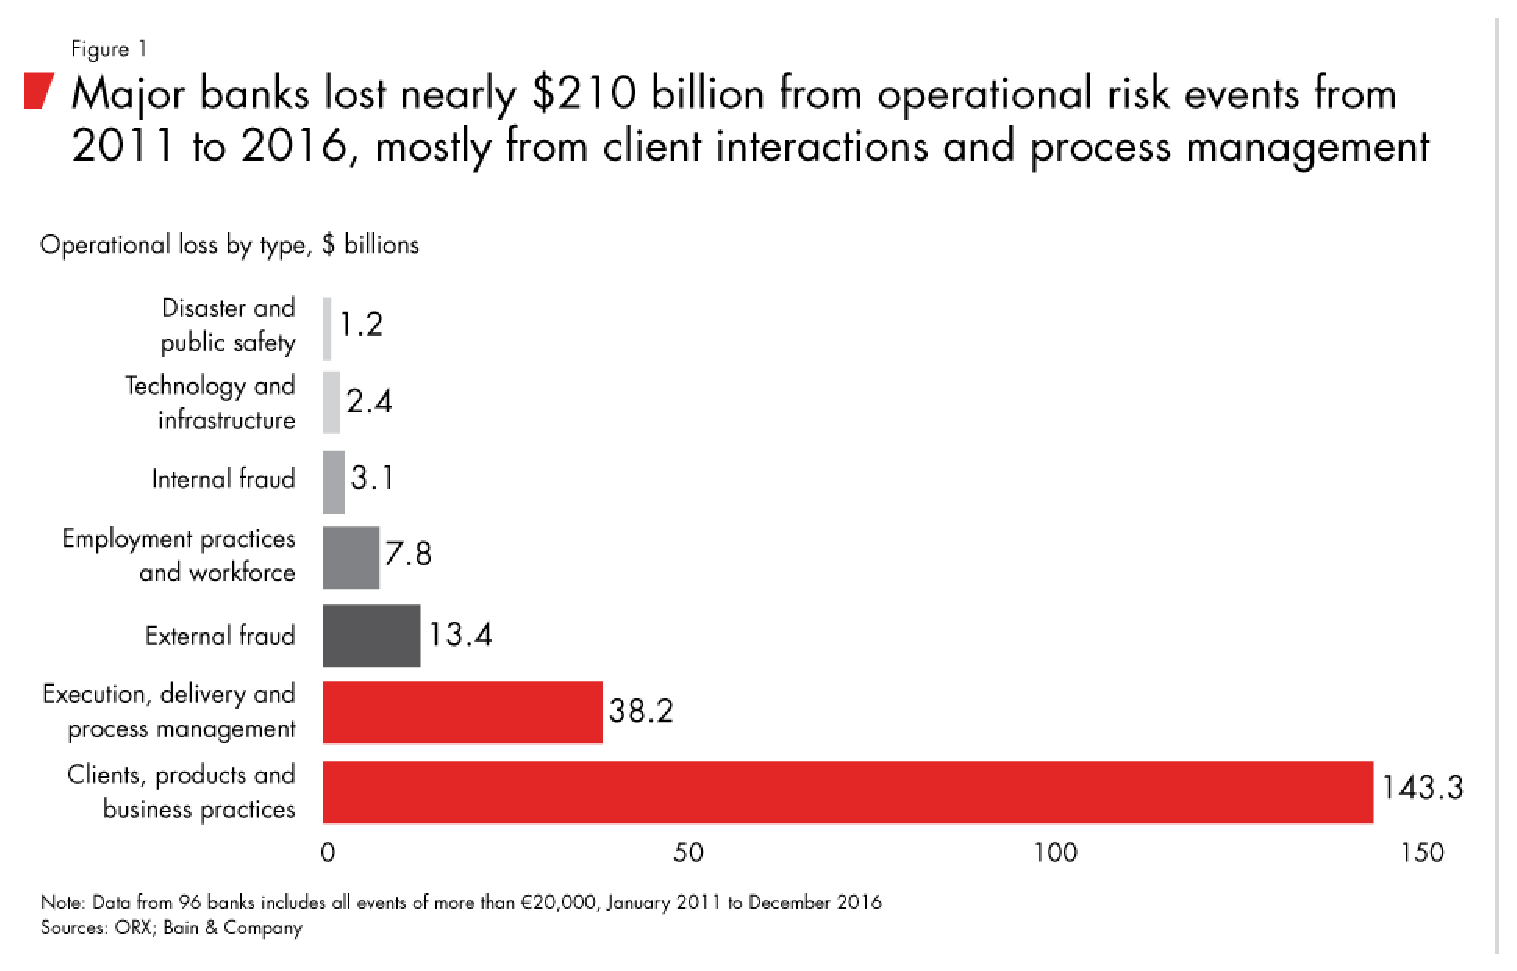
\includegraphics[width=15cm,height=10cm]{bank-oprisk_fig1_full.eps}}
             {Source: \url{https://www.bain.com/contentassets/f0199ad9887e402cb37cd1fd316f5ee3/bain_brief_how_banks_can_manage_operational_risk.pdf}}
\caption[Losses suffered from 2011 to 2016 from Oprisk]{Histogram showing a breakdown of gross losses focusing on OpRisk loss events in comparison to each other recorded from 2011 up to and including 2016}
\label{bank-oprisk_fig}
\end{figure}

In South Africa (SA), there is an upcoming case of price fixing and
market allocation in trading foreign exchange (FX) currency pairs,
reffered to the SA based competition tribunal for prosecution. Absa
bank, Standard bank \& Investec may be liable to payment of an
admistrative penalty equal to 10\% of their annual turnover in 2016,
following accusations by the local based competition commission in
February 2017, of rogue traders manipulating the price of the rand
through buying and selling US dollars in exchange for the rand at fixed
prices. According to the competition commission, it has been alleged
that currency traders have been colluding or manipulating the price of
the rand through these buy and sell orders to change supply of the
currency.\medskip

This has compromised the quality and accuracy of risk management's
advisory service and pedigree, and aroused huge interest as the value of
the rand has implications on South African's. Furthermore, this kind of
behaviour can lead to catastrophic operational losses, as with the case
for the Barings event, resulting is a mismatch between business'
expectations and the value the risk management practice was able to
deliver, which is prevalent across FI's and remains unchanged. There are
many attitudes that can potentially infect organisational processes, the
most persistent of these attitudes stem from human failings that are
exploitable {[}@barberis2003survey{]}; i.e.~humans' propensity to be
deceitful during periods of distress, thus forming a basis for a
theoretical foundation of OpRisk management.

\section{Basel Committee's quantitative operational risk management framework}
\label{sec:Basel Committee's quantitative operational risk management framework}

The Bank for International Settlements (BIS) is an organisation
consisting of a group of central bank governors and heads of supervision
of central banks around the world who represent an authority on good
risk management in banking. More specifically, the BIS oversee the
duties of the Basel Committee on Banking Supervision (BCBS)/Basel
Commitee. The role of the BCBS is to set out guidelines on international
financial regulation to cover risks in the banking sector. There have
been three banking accords from the BCBS under the supervision of the
BIS in dealing with financial regulation, viz., Basel I, Basel II \&
Basel III. These accords describe an overview of capital requirements
for financial institutions (FI's) in order to create a level playing
field, by making regulations uniform throughout the world.\medskip 

\subsection{The Capital Adequacy Accord (Basel I)}

Basel I was established in 1988. Basel I meant that FI's were required
to assign capital for credit risk to protect against credit default. In
1996, an amendment to Basel I imposed additional requirements to cover
exposure due to market risk as well as credit risks. Basel I effectively
minimised rules that favoured local FI's over potential foreign
competitors, by opening up global competition so that these banks could
buffer against international solvency. In 2001, the @risk2001supporting
consultative package provided an overview of the proposed framework for
regulatory capital (RC) charge for OpRisk. A fiancial institution (FI)
has an OpRisk component, which constitutes a substantial risk component
other than credit and market risk. There are two types of OpRisk's viz.,
potential high severity risk where the probability of an extreme loss is
very small but costly, and high frequency/low severity risk where
frequency plays a major role in the OpRisk capital charge
calculation.\medskip 

\subsection{New Capital Adequacy Accord (Basel II)}

The framework for Basel II was implemented in June 2006. The rationale
for Basel II is to introduces risk sensitivity through more restrictive
capital charge measures and flexibility with specific emphasis on
OpRisk. The structure of the new accord is built upon a three-pillar
framework: Pillar I stipulates minimum capital requirements for the
calcualtion of regulatory capital for credit risk, market risk and
OpRisk in order to retain capital to ward against these risks. Pillar II
imposes a supervisory review process through which additional
requirements can be imposed, such as the bank's internal capital
assessements, or to act on needed adequate capital support or best
practice for mitigating their risks. Pillar III relates to market
discipline, i.e.~transparency requirements which require banks to
publicly provide risk disclosures to keep them in line by enabling
investors to form an accurate view of their capital adequacy, in order
to reward or punish them on the basis of their risk profile.\medskip

\subsection{Basel III}

Basel III establishes tougher capital standards through more restrictive
capital definitions, higher RWA's, additional capital buffers, and
higher requirements for minimum capital ratios {[}@mysis2013{]}. Through
Basel III, the BCBS is introducing a number of fundamental reforms
grouped under three main headings {[}@basel2010basel{]}: 1{]} A future
of more capital through incremental trading book risk (credit items in
trading book treated in the same way as if they were in banking book),
2{]} More liquidity through the introduction of a global liquidity risk
standard (Basel III will push banks toward holding greater levels of
liquid instruments, such as government bonds and more liquid corporate
instruments), and 3{]} Lower risk under the new requirements of the
capital base, i.e., establish more standardized risk-adjusted capital
requirements.\medskip

Regarding the sequence Basel I and Basel II: Regulation begins as a
qualitative recommendation which requires banks to have an
assets-to-capital multiple of at least 20, then focuses on ratios in
which both on-balance sheet and off-balance sheet items are used to
calculate the bank's total risk-weighted assets
(RWA's)\footnote{Also reffered to as risk-weighted amount, it is a measure of the bank's total credit exposure},
then on tail risk. In other words, auditors' discretion is replaced by
market perception of capital, meaning there is a market risk capital
charge for all items in the trading business line, then exciting new
static risk management approaches which involve calculating a 99.9
percentile left tail confidence interval to measure OpRisk value-at-risk
(VaR) and convert it into a RC charge.\medskip 

The future regulatory environment requires OpRisk professionals, who are
not only intelligent, creative and motivated but also have the courage
to uphold the OpRisk advisory service standards. Businesses that want to
successfuly manage risk, would be well advised to utilize new
theoretical and empirical techniques, such that large and small scale
experiments play an important role in risk analysis and regulatory
research.

\section{Modern OpRisk measurement frameworks (ORMF's)}
\label{sec:modern OpRisk measurement frameworks (ORMF's)}

Basel II describes three methods of calculating capital charge for
OpRisk RC viz., the standardised approach (SA), the basic indicator
approach (BIA) and the internal measurement approach (IMA). The basic
indicator approach (BIA) sets the OpRisk RC equal to a percentage (15\%)
of the annual gross income of the firm as a whole to determine the
annual capital charge. The SA is similar to the BIA except the firm is
split into eight business lines and assigned a different percentage of a
three year average gross income per business line, the summation of
which is the capital charge {[}@hoohlo2015new{]}. In the IMA, the bank
uses it's own internal models to calculate OpRisk loss.\medskip

\subsection{Advanced Measurement Approach (AMA)}

The advanced measurement approach (AMA) is an IMA method which applies
estimation techniques of OpRisk capital charge derived from a bank's
internal risk measurement system @cruz2002modeling. Basel II proposed
measurement of OpRisk to define capital requirements against unexpected
bank losses whereas the unexpected loss (UL) is the quantile for the
level \(\alpha\) minus the mean. According to the AMA, which is thought
to outperform the simpler SA approach and the BIA, RC requirements are
defined according to the UL limit in one year and the loss distribution
at a 99.9\% confidence level (\(\alpha = 0.01\%\)) aggegate loss
distribution\footnote{The aggregate loss distribution is obtained by convoluting a loss event frequency distribution and a loss severity distribution by means of the random sums method.}
used as a measure of RC. The BCBS proposes to define RC as \(RC = UL\).
This involves simulations based on historical data to establish
frequency and severity distributions for losses. In this case the RC is
a VaR measure.\medskip

The Basel III capital adequacy rules permit model-based calculation
methods for capital, including the AMA for OpRisk capital. Under Basel
III, standardised methods for OpRisk capital have been overhauled,
however for a while there was no prospect of an overhaul of the AMA.
Given the relative infancy of the field of OpRisk measurement, banks are
mostly free to choose among various AMA principle-based frameworks to a
significant degree of flexibility {[}@risk2016supporting{]}. A bank that
undertakes an AMA should be able to influence their capital requirements
through modeling techniques resulting in lowered pressure on OpRisk
capital levels, which in turn has a positive impact on the bank.\medskip

A FI's ability to determine the framework used for its regulatory OpRisk
RC calculation, evolves from how advanced the FI is along the spectrum
of available approaches used to determine capital charge
{[}@risk2001supporting{]}. BCBS recognizes that a variety of potentially
credible approaches to quantify OpRisk are currently being developed by
the industry, and that these R\&D activities should be incentivised.
Increasing levels of sophistication of OpRisk measurement methodologies
should generally be rewarded with a reduction in the regulatory OpRisk
capital requirement.

\subsection{The standardised measurement approach (SMA)}

The flexibility of internal models was expected to narrow over time as
more accurate OpRisk measurement was obtained and stable measures of RC
were reached, ultimately leading to the emergence of best practice.
Instead, internal models produced wildly differing results of OpRisk RC
capital from bank to bank, contrary to the expectations of the BCBS. In
March 2016, the BCBS published for consultation a standardised
measurement approach (SMA) for OpRisk RC; that proposes to abandon the
freedom of internal modelling (thus ending the AMA) approaches for
OpRisk RC, in exchange for being able to use a simple formula to
facilitate comparability across the industry.\medskip

Under the SMA, RC will be determined using a simple method comprising of
two components: A stylised systemic risk model (business indicator
component), and an idiosyncratic risk model (loss component), which are
combined via an internal loss multiplier (ILM), whose function is to
link capital to a FI's operational loss experience to determine SMA
capital.\medskip

The SMA formula is thought to be consistent with regulators' intent for
simplification and increased comparability across most banks. However,
there is a feeling from some in the banking industry that the SMA is
disadvantaged as it is not the same as measuring OpRisk.
@mignola2016comments and @peters2016should identified that the SMA does
not respond appropriately to changes in the risk profile of a bank i.e.,
it is unstable viz., two banks of the same risk profile and size can
exibit OpRisk RC differences exceeding 100\%, and risk insensitive; that
SMA capital results generally appear to be more variable across banks
than AMA results, where banks had the option of fitting the loss data to
statistical distributions.

\subsection{Argument}
\label{ssec:Argument}

Over the last twenty years, hard-won incremental steps to develop a
measure for the size of OpRisk exposure along with the emergence of
promising technologies presents a unique opportunity for bankers and
treasurers - traditionally risk-averse players - to develop a novel type
of way of looking at decision making under risk/uncertainty. New
technologies have been introduced which make use of up to date technical
solutions (such as homo heuristics developed by @gigerenzer2009homo, who
mainatain their methods solve practical finance problems by simple rules
of thumb, or @kahneman2003perspective's intuitive judgements and
deliberate decision making), argued to more likely represent the true
embedded OpRisk in financial organisations as these methods are designed
to fit normal behavioral patterns in their formulation, which is
consistent with how decisions are made under risk/uncertainty.\medskip 

What are the important steps toward completing the post crisis reforms
during the current year? Should the risk management fraternity follow
the
chartered\footnote{Meaning as of the publication [@risk2016supporting] the methods brought forth in the consultative document have not been approved for the public, the ideas within an experimental (leased) phase for the exclusive use of BCBS and certain FI's}
path followed in the @risk2016supporting consultative document,
scrapping away twenty years of internal measurement approaches (such as
the AMA), or should the focus of financial regulators shift toward
improving on what they see fit within current existing AMA frameworks.
The question is should OpRisk managements' focus be on stimulating
active discussions on practical approaches to quantify, model and manage
OpRisk for better risk management and improved controls, or abandon the
adoption of innovative measurement approaches, such as the AMA, in
exchange for being able to use a simple formula across the whole
industry?\medskip 

\section{Context of the study}
\label{sec:Context of the study}

Regulatory reforms are designed and fines imposed to protect against
operational errors and other conduct costs connected with wrongdoing and
employee misconduct. Despite the introduction and use of these seemingly
robust strategies, regulations, processes and practices relating to
managing risk in FI's, bank losses continue to occur at a rather
distressing frequency. A cyclical pattern of OpRisk loss events still
persists; as evidenced in the recent price fixing and collusion cases,
defeating the explicit objectives of risk management frameworks. This
demonstrates a scourge of reflexivity prevailing in financial markets
emphasising that, there are theories that seem to work for a time only
to outlive their use and become insufficient for the complexities that
arise in reality.\medskip 

\subsection{Why \texttt{OpRisk?}}

A forceful narrative in management theory is that an organisation
running effective maintenance procedures combined with optimal team and
individual performers i.e., the right balance of skills in the labour
force and adequate technological advancements, means systems and
services can be used to more efficiently produce material gains, enhance
organisational effectiveness, meet business objectives and increase
investment activity. Conversely, the risk of the loss of business
certainty associated with lowered organisational competitiveness and
inadequate systems technology that underpins operations and services is
a key source leading to a potential breakdown in investment services
activity {[}@hoohlo2015new{]}. In fact OpRisk control could set banks
apart in competition. This serves as an incentive to support regulation,
particularly Basel III recovery and resolution processes.\medskip

Consider the case of a regulator in a financial system, who assumes that
he/she is consiously and accurately analysing an observed subject,
trusting the validity and relying on the visual information that their
sense of sight reveals. In the absence of visual confirmation they are
hindered from extracting and/or analysing information about the system
and their efforts to regulate could potentialy fail. The organisational
methods and functioning of current information systems in this industry
sector obscure the full extent of OpRisk challenges from the eyes of the
risk practitioner.\medskip 

When an attack such as an operational error occurs at a speed that the
OpRisk agent (an individual legal entity or a group) is unable to react
quickly enough, due to limitations of their processing speed, and they
are not able to process all the information in the given time span, they
could lose control/fail to comply with regulatory standards. The latter
case is more often than not the most accurate reflection of current risk
management practices. The agent represents one end of the spectrum of a
risk management strategy, which mitigates risk and enforces regulation,
dependent on the information recieved. The other end of the spectrum is
one which does not react at all to changes in the system
environment.\medskip 

Current conventional financial systems where information processing is
slow and have a tendency to rely on manual, uncertain, unpredictable and
unrealistic controls, obscure risk management reporting and produce
undesirable market conditions. The OpRisk management function should be
able to assist the firms' ability to mitigate risks by acquiring and/or
refining risk management solutions which deliver reliable and consistent
benefits of improved control and management of the risks inherent in
banking operations {[}@mysis2013{]}. This proposal attempts to fill the
gap in the current system where there is a risk management information
lag or an obstruction from the eyes of the risk practitioner.

\section{Analysis and interpretation issues with behavioral finance theory}
\label{sec:Analysis and interpretation issues with behavioral finance theory}

Behavioral management theory is very much concerned with social factors
such as motivation, support and employee relations. A critical component
of behavioral finance is building models which better reflect actual
behavior. Studies have revealed that these social factors are not easy
to incorporate into finance models or to understand in the traditional
framework.\medskip 

The traditional finance paradigm seeks to understand financial markets
using models in which agents are \lq\lq rational\rq\rq. According to
@barberis2003survey, this means that agents update their beliefs on the
onset of new information, and that given their beliefs, they make
choices that are normatively acceptable, and that most people do this
most of the time. Neoclassical theory has grown to become the primary
take on modern-day economics formed to solve problems for decision
making under uncertainty/risk. Expected Utility Theory (EUT) has
dominated the analysis and has been generally accepted as the normative
model of rational choice, and widely applied as a descriptive model of
economic choice {[}@kahneman2013prospect{]}.

\subsection{Expected utility theory}
\label{ssec:Expected utility theory}

Expected utility
theory\footnote{Expected utility theory provides a model of rationality based on choice.}
(EUT): We see a fundamental relation for expected utility (Expectation)
of a contract \(X\), that yields outcome \(x_i\) with probability
\(p_i\), where \(X = (x_1,p_1; ...; x_n,p_n)\) and
\(p_1+p_2+\ldots+p_n=1\) given by:

\singlespacing

\begin{equation}\label{EUT_extended}
U(x_1,p_1;\ldots;x_n,p_n) = p_1u(x_1)+\ldots+p_nu(x_n) 
\end{equation} \doublespacing corroborated by @morgenstern1953theory;
@friedman1948utility; @kahneman2013prospect \& others.

A common thread running through the rational viz., the neoclassical take
of modern-day economics vs the non-neoclassical schools of thought are
findings of behavioral economics which tend to refute the notion that
individuals behave rationally. Many argue that individuals are
fundamentally irrational because they do not behave rationally giving
rise to a literature and debates as to which heuristics and sociological
and institutional priors are rational
{[}@altman2008behavioral{]}.\medskip

In the real world there is a point of transition between the traditional
(neoclassical) approach to decision making, based on data and data
anaysis (logic and rational), by adding new parameters and arguments
that are outside rational conventional thinking but are also valid. For
example, that neoclassical theory makes use of the assumption that all
parties will behave rationally overlooks the fact that human nature is
vulnerable to other forces, which causes people to make irrational
choices.\medskip 

An essential ingredient of any model trying to understand trading
behavior is an assumption about investor preferences
{[}@barberis2003survey{]}, or how investors evaluate risky gambles.
Investors systematically deviate from rationality when making financial
decisions, yet as acknowledged by @kuhnen2005neural, the mechanisms
responsible for these deviations have not been fully identified. Some
errors in judgement suggest distinct mental operations promote different
types of financial choices that may lead to investing mistakes.
Deviations from the optimal investment strategy of a rational risk
neutral agent are viewed as risk-seeking mistakes and risk-aversion
mistakes {[}@kuhnen2005neural{]}.\medskip 

\subsection{Theoretical investigations for the quantification of moderm ORMF}

@kuhnen2005neural explain that these risk-seeking choices (such as
gambling at a casino) and risk-averse choices (such as buying insurance)
may be driven by distinct
neural\footnote{As recent evidence from human brain imaging has shown [@kuhnen2005neural] linking neural states to risk-related behaviours [@paulus2003increased].}
phenomena, which when activated can lead to a shift in risk preferences.
@kuhnen2005neural found that certain areas of the brain precede
risk-seeking mistakes or risky choices and other areas precede
risk-aversion mistakes or riskless choices. A risk-aversion mistake is
one where a gamble on a prospect of a gain is taken by a risk-averse
agent in the face of the chance of a prospective loss. The fear of
losing prohibits one's urge to gamble, but people engage in gambling
activity anyway. @barberis2003survey show that people regularly deviate
from the traditional finance paradigm evidenced by the extensive
experimental results compiled by cognitive psycologists on how people
make decisions given their beliefs.\medskip 

@kahneman2013prospect maintains, preferences between prospects which
violate rational behaviour demonstrate that outcomes which are obtained
with certainty are overweighted relative to uncertain outcomes. This
will contribute to a risk-averse preference for a sure gain over a
larger gain that is merely probable or a risk-seeking preference for a
loss that is merely probable over a smaller loss that it certain. As a
psycological principle, overweighting of certainty favours risk-aversion
in the domain of gains and risk-seeking in the domain of losses.\medskip

The present discussion replicates the common behavioral pattern of risk
aversion, where people weigh losses more than equivalent gains.
Furthermore, neuroeconomic research shows that this pattern of behavior
is directly tied to the brain's greater sensitivity to potential losses
than gains {[}@tom2007neural{]}. This provides a target for
investigating a more comprehensive theory of individual decision-making
rather than the rational actor model and thus yield new insights
relevant to economic
theory\footnote{Representing ability of FI's financial market models to characterise the repeated decision-making process that applies to loss aversion}
{[}@kuhnen2005neural{]}.\medskip  

If people are reasonably accurate in predicting their choices, the
presence of systematic violations of risk neutral behavior provides
presumptive evidence against this i.e., people systematically violate
EUT when choosing among risky gambles. This seeks to improve and adapt
to reality and advance different interpretations of economic behaviour;
viz., to propose a more adequately descriptive model, that can represent
the basis for an alternative to the way the traditional model is built
for decisions taken under uncertainty. This has led some influential
commentators to call for an entirely new economic paradigm to displace
conventional neoclassical theory with a psycologically more realistic
preference specification {[}@list2004neoclassical{]}.

\section{A new class of ORMF models approach}
\label{sec:A new class of ORMF models approach}

A substantial body of evidence shows that decision makers systematically
violate EUT when choosing between risky prospects. Indeed, people would
rather satisfy their needs than maximise their utility, contravening the
normative model of rational choice (i.e., EUT) which has dominated the
analysis of decision making under risk. In recent work
{[}@barberis2003survey{]} in behavioral finance, it has been argued that
some of the lessons learnt from violations of EUT are central to
understanding a number of financial phenomena. In response to this,
there has been several theories put forward advocating for the basis of
a slightly different intepretation which describes how individuals
actually make decisions under uncertainty/risk. Of all the non-EUT's, we
focus on Prospect Theory (PT) as this framework has had most success
matching most empirical
facts\footnote{OpRisk loss events in FI's are largely due to human failings that are exploitable e.g., fraudulent trading activity, and PT is based on the same behavioural element of how people make financial decisions about prospects}.\medskip 

@kahneman2013prospect list the key elements of PT, which are 1{]} a
value function, and 2{]} a non-linear transformation of the probability
scale, that factors in risk aversion of the participants. According to
@kahneman2013prospect, the probability scale overweights small
probabilities and underweights high probabilities. This feature is known
as loss/risk aversion: This means that people have a greater sensitivity
to losses (around 2.5 times more times) than gains, and are especially
sensitive to small losses unless accompanied by small
gains\footnote{Diminishing marginal utility for gains but opposite for losses.}.
Loss aversion is a strong differentiator when it comes to explaining
exceptions to the general risk patterns that characterize prospect
theory.\medskip 

\subsection{Prospect theory}
\label{ssec:Prospect theory}

By relaxation of the expectation principle in equation
\ref{ssec:Expected utility theory}, the over-all value
\(\mathbf{\bigvee}\) of the regular prospect \((x,p;y,q)\): In such a
prospect, one receives \(x\) with probability \(p\), \(y\) with
probability \(q\), and nothing with probability \(1-p-q\), is expressed
in terms of two scales, \(\pi(\cdot)\), and \(\nu(\cdot)\), where
\(\pi(\cdot)\) is a decision weight and \(\nu(\cdot)\) a number
reflecting the subjective value of the outcome. Then
\(\mathbf{\bigvee}\) is assigned the value:

\begin{equation}\label{eqn2}
\mathbf{\bigvee}=\pi(p)\nu(x)+\pi(q)\nu(y) \qquad\mbox{iff} \qquad p+q \leq 1
\end{equation}

The scale, \(\pi\), associates with each probability \(p\) a decision
weight which reflects the impact of \(p\) on the over-all value of the
prospect. The second scale, \(\nu\), assigns to each outcome \(x\) a
number \(\nu(x)\), which measures the value of deviations from a
reference point i.e., gains or losses. \(\pi\) is not a probability
measure and \(\pi(p) + \pi(1-p) < 1\). Through PT we add new parameters
and arguments to improve the mathematical modelling method for decisions
taken under risk/uncertainty, such that the value of each outcome is
multiplied by a decision weight, not by an additive probability.

PT looks for common attitudes in people (in FI's) with regard to their
behaviour toward taking financial risks or gambles that cannot be
captured by EUT. In light of this view, people are not fully invested in
either of the percieved outcomes \(x\) and \(y\), Which tells us that
\(p+q \leq 1\). In lieu of this, an FI using (internal) historical
OpRisk loss data to model future events; say a historical case of fraud
at the FI occurs and is incorporated in the model, the probability of
making the same error in future is provided for in the model versus risk
events that haven't happened. The modelled future should over-provide
for the loss events that have already occured, which fits normal
patterns around individuals psycological make up and is consistent with
risk-averse behavior. The idea at the basis of PT is that a better
modeling method can be obtained which leads to a closer approximation of
the over-all-value of OpRisk losses.

\subsection{Modeling}

In this study, an important new algorithm for ORMFs and is laid out
coupled with data intensive estimation techniques; viz.~Generalised
Additive Models for locatin Scale \& Shape (GAMLSS), Generalized Linear
Models (GLDs), Artificial Neural Networks (ANNs), Random Forest (RF) \&
Decision Trees (DTs), which have capabilities to tease out the deep
hierarchies in the features of covariates irrespective of the challenges
associated with the non-linear or multi-dimensional nature of the
underlying problem, at the same time supporting the call from industry
for a new class of EBOR models that capture forward-looking aspects.
Machine Learning (ML) is used as a substitute tool for the traditional
model based Autoregressive Moving Average (ARMA) used for analysing and
representing stochastic processes. As opposed to the statistical tool,
ML does not impose a functional relationship between variables, the
functional relationship is determined by extracting the pattern of the
training set and by learning from the data observed.\medskip 

Using computationally intensive (using ML techniques on historical data
) OpRisk measurement techniques and mixing with a theory is not a new
approach for modeling, particularly in calculating OpRisk RC; as
evidenced through @agostini2010combining in a study whereby the LDA
model for forecasting OpRisk RC, via VaR, was implemented in conjunction
with the use of advanced credibility theory (CT). The idea at the basis
of their use of CT, is to advance the very recent literature that a
better estimation of the OpRisk RC measurement can be obtained by
integrating historical data and scenario analysis i.e., combining the
historical simulations with scenario assessments through formulas that
are weighted averages of the historical data entries and scenario
assessments, advocating for the combined use of both
experiences.\medskip 

However, applying ML is an original way of looking at the approximation
issue as opposed to advanced CT. The essential feature of PT are
assumptions which are more compatible with basic principles of
perception and judgement for decisions taken under uncertainty, whereas
ML will reveal additional chance probabilities determined through the
natural clusters of unknown data feature findings from which new
discoveries are made.\medskip

According to @kahneman2013prospect, the decision maker, who is a risk
agent within the FI, constructs a representation of the losses and
outcomes that are relevant to the decision, then assesses the value of
each prospect and chooses according to the losses (changes in wealth),
not the overall financial state of the FI. We wish to bring the
prescribed model to equilibrium, by applying a method that tries to
establish what accurately ascribes to decision rules that people wish to
obey, in made predictions about what operational loss events might
result in the future, then use empirical data to test this idea in a way
that is falsifyable.

\section{Problem statement}
\label{sec:Problem statement}

\subsection{Main problem}

The existing models of OpRisk VaR measurement frameworks assume FI's are
risk neutral, and do not learn from past losses/mistakes: We address
weaknesses in current OpRisk VaR measurement frameworks by assuming that
FI's are more risk averse. Furthermore, introducing exposure-based
operational risk modeling, we gain an understanding of how capturing
past losses and exposures of forward looking aspects affect risk
attitudes using machine learning techniques. As a consequence, projected
future losses are estimated through a learning algorithm adapting
capital estimates to changes in the risk profile, i.e.~in the
introduction of new products or changes in the business mix of the
portfolio (e.g.~mergers, trade terminatons, allocations or
disinvestments), providing sufficient incentives for OpRisk management
to mitigate risk.

\section{Objectives of the study}
\label{sec:Objectives of the study}

The research objectives are three-fold:

\subsection{Exposure-based OpRisk (EBOR) models}

To quantify OpRisk losses by introducing generalised additive models for
location, scale and shape (GAMLSS) in the framework for OpRisk
management, that captures exposures to forward-looking aspects of the
OpRisk loss prediction problem. EBOR treatments effectively replace
historical loss severity curves obtained from historical loss counts, by
looking into deep hierarchies in the features of covariates in
investment banking (IB), and by forward-looking measures using event
frequencies based on actual operational risk (OpRisk) exposures in the
business environment and internal control risk factors (BEICF) thereof.

\subsection{Modeling OpRisk depending on covariates}

To investigate the performance of several supervised learning classes of
data-intensive methodologies for the improved assessment of OpRisk
against current \emph{traditional} statistical estimation techniques.
Three different machine learning techniques viz., DTs, RFs, and ANNs,
are employed to approximate weights of input features (the risk factors)
of the model. A comprehensive list of user defined input variables with
associated root causes contribute to the \emph{frequency} of OpRisk
events of the underlying value-adding processes. Moreover, the
\emph{severity} of OpRisk is also borne out through loss impacts in the
dataset . As a consequence of theses new mwthodologies, capital
estimates should be able to adapt to changes in the risk profile of the
bank, i.e.~upon the addition of new products or varying the business mix
of the bank providing sufficient incentives for ORMF to mitigate risk
{[}@einemann2018operational{]}.

\subsection{Interpretation Issues using cluster analysis}

To identify potential flaws in the mathematical framework for the loss
distribution approach (LDA) model of ORM, which is based the derivation
of OpRisk losses based on a risk-neutral measure \(\mathbb{Q}\), by
employing Cluster Analysis (CA). The study addresses weaknesses in the
current \emph{traditional} LDA model framework, by assuming managerial
risk-taking attitudes are more risk averse. More precisely, CA learns
the deep hierarchies of input
features\footnote{A typical approach taken in the literature is to use an unsupervised learning algorithm to train a model of the unlabeled data and then use the results to extract interesting features from the data [@coates2012learning]}
that constitute OpRisk event \emph{frequencies} \& \emph{severities} of
losses during banking operations. In theory, a risk manager who
experiences persistent/excessive losses due to particular risk events,
would over-compensate cover for these particular risk types. This would
show in reduced losses in those loss event types over time, subsequently
determining whether risk adverse techniques over-compensate for
persistent losses.

\section{Significance of the study}
\label{sec:Significance of the study}

This study fills a gap in that advancing OpRisk VaR measurement methods
beyond simplistic and traditional techniques, new data-intensive
techniques offer an important tool for ORMFs and at the same time
supporting the call from industry for a new class of EBOR models that
capture forward-looking aspects of ORM {[}@embrechts2018modeling{]}. The
current \emph{traditional} approach consists of a loss data collection
exercise (LDCE) which suffers from inadequate technologies at times
relying on spreadsheets and manual controls to pull numbers together,
and therefore do not support the use of data intensive techniques for
the management of financial risks. In this study, a new dataset with
unique feature characteristics is developed using an automated LDCE, as
defined by @basel2011operational for internal data. The dataset in
question is at the level of individual loss events, it is fundamental as
part of the study to know when they happened, and be able to identify
the root causes of losses arising from which OpRisk loss
events.\medskip 

This study will provide guidance on combining various supervised
learning techniques with extreme value theory (EVT) fitting, which is
very much based on the Dynamic EVT-POT model developed by
@chavez2016extreme. This can only happen due to an abundance of larger
and better quality datasets and which also benefits the loss
distribution approach (LDA) and other areas of OpRisk modeling. In
@chavez2016extreme, they consider dynamic models based on covariates and
in particular concentrate on the influence of internal root causes that
prove to be useful from the proposed methodology. Moreover, EBOR models
are important due to wide applicability beyond capital calculation and
the potential to evolve into an important tool for auditing process and
early detection of potential losses, culminating in structural and
operational changes in the FI, hence releasing human capital to focus on
dilemmas that require human judgement.

\section{Organisation of the study}
\label{sec:Organisation of the study}

This study is made up of seven chapters. The introductory chapter is to
the purpose, overview, research problem \& objectives, and the
significance of the study. The introductory chapter is succeded by a
general literaty review chapter (two) followed by three stand alone
chapters each focusing on the three research objectives regarding the
issues in OpRisk capital requirement estimation.\medskip

Chapter one begins with an account of significance and a commentary on
the nature and scope of the practical problem. It then provides a
background of current issues when dealing with OpRisk measurement, the
research problem and research questions thereof. Chapter two gives an
overview of the literature concerning the LDA, an AMA technique used in
the generation of \texttt{OpVaR}. It concludes by proposing the a
research methodology in which a combination of ML techniques and
statistical theory underlying ORMF's would benefit measurement of
capital requirements for OpVaR.\medskip

Chapter three looks at the methodological and empirical determinants of
OpRisk measurement. It explores the different dataset\ldots{}


\end{document}
